\documentclass[a4paper,10pt]{article}
\usepackage[hidelinks]{hyperref}
\def\UrlBreaks{\do\/\do-} % breaks long url in references
\usepackage{graphicx}
\usepackage[english]{babel}
\usepackage{listings}
\usepackage[labelfont=it,textfont={it},singlelinecheck=on,justification=centering]{caption}
\DeclareGraphicsExtensions{.pdf,.png,.jpg}
\begin{document}
\lstset{basicstyle=\ttfamily\footnotesize,breaklines=true}
\lstset{numbers=left, numberstyle=\tiny, stepnumber=1, numbersep=5pt}
\lstset{language=TeX}


\title{\large \bf Metadisk:  Blockchain-Based Decentralized File Storage Application}
\author{\small Shawn Wilkinson + Jim Lowry\\ \small shawn@storj.io + jim@storj.io \\  \small \url{http://storj.io} \\  \small \url{http://metadisk.org}}
\maketitle

%\section{Abstract}

\begin{abstract}
Metadisk is an open source software project seeking to prove conceptually that cloud storage applications can be made more decentralized, more secure, and more efficient. In addition, Metadisk provides a prototyping platform for a fully decentralized network. In pursuit of this goal, we propose developing a web application that provides an interface for non-technical users, and an underlying API for native applications and feature extensions. A cryptocurrency will serve as both an incentive and payment mechanism while a separate blockchain will be used as a datastore for file metadata. This application will seek to operate autonomously as a peer-to-peer network of nodes running open-source code, depending on a public blockchain for information rather than a central database. Metadisk’s primary objective is to provide a stable testing platform for a peer-to-peer cloud storage network called Storj. Metadisk’s ultimate objective is to provide a set of tools that will allow Storj to integrate more easily with traditional platforms and users. 
\end{abstract}
\section{Introduction}

“Cloud storage” is a marketing term that exploits the popular craving for novelty. It has caught on because, to ordinary users, “the cloud” sounds like a newer technology when compared to “the internet,” “client-server,” or “as a service.” This rebranding of existing technology is simple misdirection, not magic.  When data is stored “in the cloud,” it is transferred over TCP/IP from the client’s computer to the host’s server in a data center.  It is the same old client-server model that has existed since the days of the mainframe and dumb terminal. That server then copies it to other servers to comply with industry-standard redundancy policies whereby three copies are made. The current model of cloud storage that operates through centralized institutions that are entrusted with private information is inherently insecure in many ways.  Information thieves, spies, and censors can copy or destroy data stored on the host servers through political strategy, legal tactics, and technological means.  \\

\begin{figure}[h!]
  \centering
      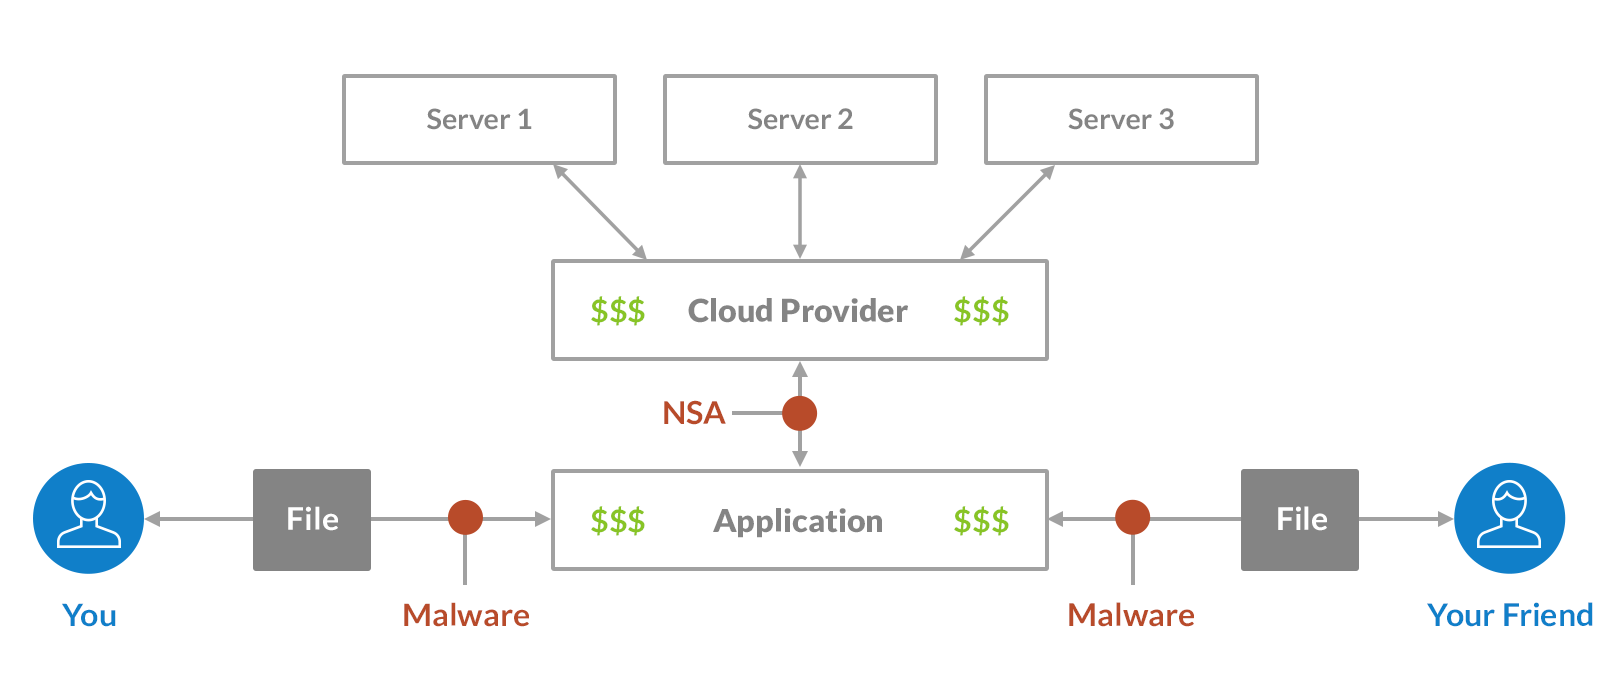
\includegraphics[width=\linewidth]{01}
  \caption{The Standard Model for Cloud Applications}
\end{figure}

The distinction between these three categories has become increasingly blurry over time. It is now clear that personal privacy and enterprise information security can only be achieved if off-site data stores can be protected from attacks originating in and operating through each category.  Having easily identifiable central points of attack built into the model is a problem solvable through decentralization and automation. Other inherent security flaws in the current cloud storage model are the types of payment mechanisms currently in widespread use by cloud storage services.  These mechanisms are neither private nor information-secure because most online payment technologies store and leak information about the payer and payee.\\

We need a cloud storage model that is not based on trust between client and host.  All client private data, including filename, date and other metadata, must be encrypted before any transfer takes place from a client’s computer to the cloud.  There can be no centralized point of attack using political or legal attack vectors.  All incentive payments for both resource providers and consumers will be automated and made in a pseudonymous cryptocurrency.  It is time for the cloud to truly become a cloud, made up of a vast multitude of resource droplets that are added and subtracted as the cloud forms, moves, and changes shape.\\

The overarching design principles enabling a decentralized storage network have been known for several years. Projects like MaidSafe \cite{1} and Tornet \cite{2} have outlined possible solutions. Unfortunately, achieving the security, scalability, and cost efficiency of a truly decentralized storage system will require software of immense technical complexity.  We must design the nodes and network in an extremely secure manner as we can trust neither the lines of communication nor the nodes themselves. Nodes on the network must collaborate to achieve the level of redundancy and performance of current centralized networks.  Furthermore, the software must run by itself and without manual intervention in both practical or economical aspects, i.e. in an unmanaged environment, which is a major departure from current cloud networks.      \\

These principles are achievable using a combination of existing technologies such as BitTorrent Sync \cite{3}, Bitcoin \cite{4}, public key encryption, and cryptographic hash functions.  Metadisk aims to simplify the development of a decentralized storage network by allowing integration with existing open-source projects in a modular fashion.  Such a network must be built incrementally, and with software that consists of interoperable, easily replaceable modules which support a wide variety of hardware, including the hardware-as-a-service model that existing cloud storage service providers offer. \\

Metadisk can use an incentive model similar to that employed by Bitcoin. Where bitcoin miners are paid block rewards for contributing cryptographic hashing power resources to the network, Metadisk can use its own cryptocurrency as a means to pay for and exchange storage space and bandwidth. This model harnesses the powerful free-market force of self-interest to drive the network’s growth and efficiency while remaining decentralized.  For example, if another faster method of file transfer is discovered, the network will gravitate toward that method until someone produces an even faster method. Nodes must be able to work in a constantly changing and competitive environment. 


\section{Overview}

Metadisk serves as the non-technical user interface as well as development platform for the Storj network. Using the Metadisk web interface or API, users may securely upload and download their files from the network. Files are encrypted, client-side, during the upload process using the private key provided by the user.  If a user has not used Metadisk before, the web interface may offer to assist the user in generating a private key. Metadisk communicates with the network to find available storage resources, then transfers the file to at least three (3) separate locations to maintain the three times (3x) redundancy considered the industry standard for cloud storage. The user or application can add further redundancy at an extra cost. \\

We have devised a record-keeping method that offers efficient functionality for the blockchain as a data store—thus when a user uploads a file, a record of the upload is made in a blockchain. This feature will be explained in further detail later in the section titled “Blockchain as a Metadata Store.”\\

After the file is encrypted, we find the SHA-256 hash, which serves as both a unique identifier and a way to detect file tampering.  If any alteration of the file occurs after it is uploaded, the hash will be different. We make use of this fact in the underlying platform Storj \cite{7} so the network can spot check the files without having to access them directly. A client can also using hashing to ensure that received files are authentic. The hash will be stored in a blockchain entry along with the 3× storage locations of the file used to generate the hash.  All metadata inserted into the blockchain can be protected from unauthorized reading and copying by the use of public key encryption.  Because all data and metadata entering the network is encrypted, and we can verify data through hashing, malicious entities cannot spy on, fake, or modify the data.

\begin{figure}[h!]
  \centering
      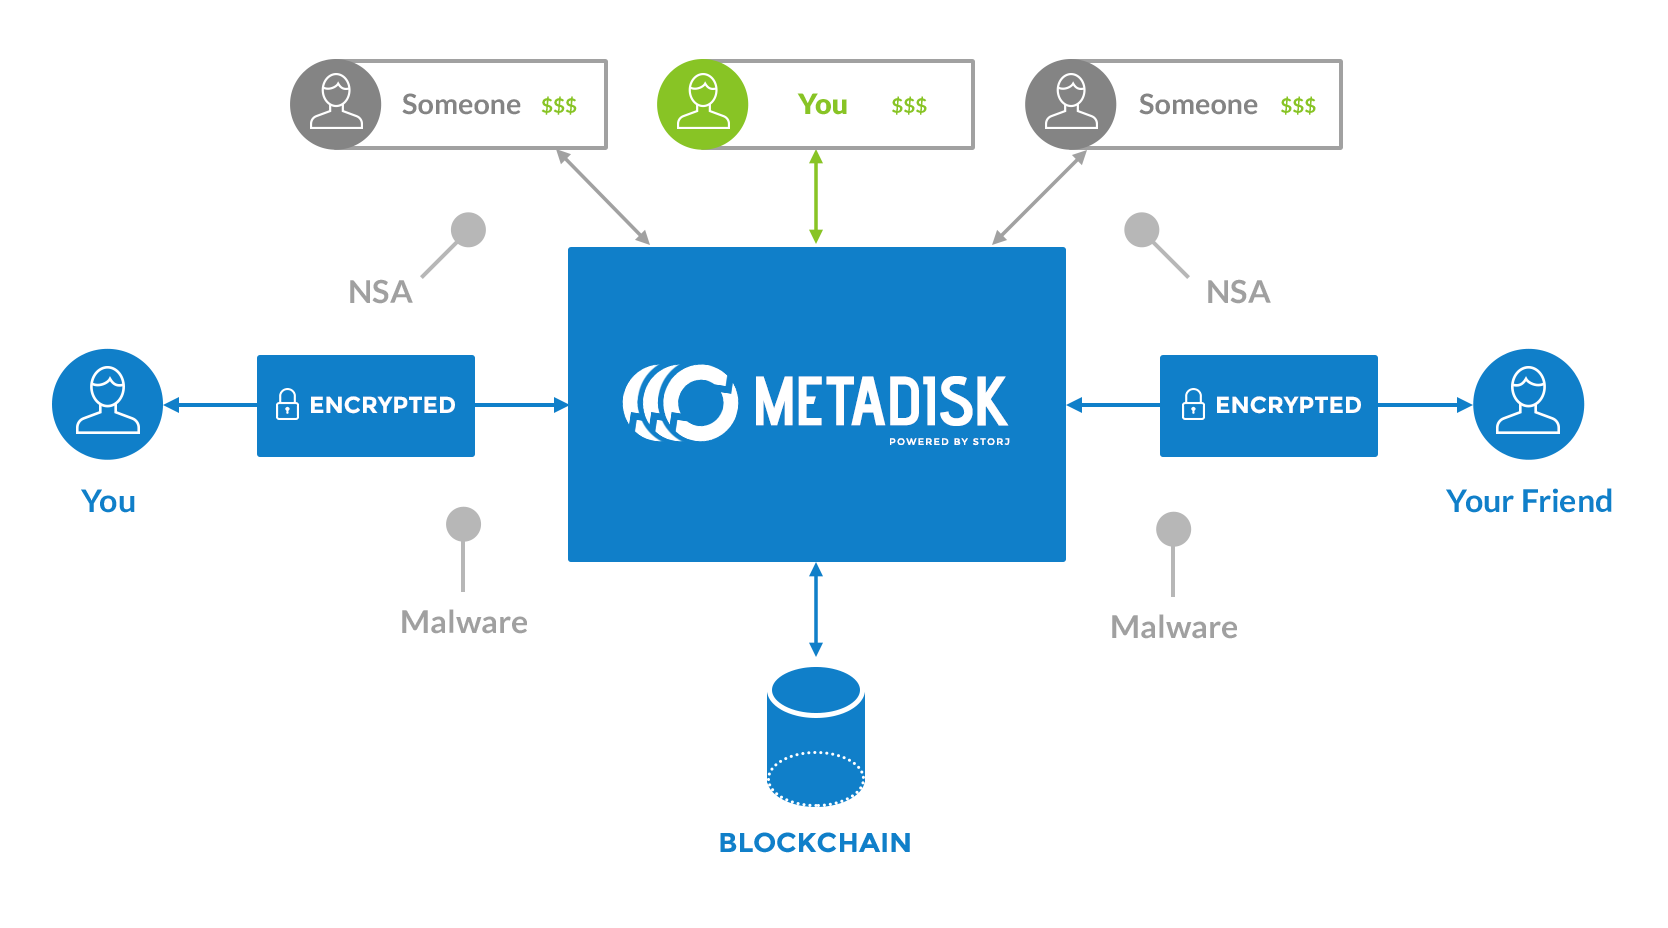
\includegraphics[width=\linewidth]{02}
  \caption{Metadisk Model of Data Storage}
\end{figure}

\subsection{Security}

Only the user has access to the decryption keys for a particular file. Furthermore, the hash of the file used to identify the file while in storage is created after the file is encrypted to keep the file contents secure. Therefore, an attacker cannot verify the contents of a file on the network, even if the existence of the file may be known. Since the file is encrypted before transmission, Metadisk is also resistant to man-in-the-middle attacks and may be used on any communication network, including open unencrypted Wifi networks.   \\

Metadisk can add client side encryption to further secure data, but it is debatable whether in-browser cryptography is actually secure \cite{5}. For non-private or insensitive files the traditional model is sufficient. For anything else, it is recommended that the files be encrypted, and passed through the API. In that way, complete failure of in browser cryptography, and a completely compromised Metadisk node will have no effect on file security. This can easily be achieved through additional native applications and toolsets.  

\subsection{Redundancy}

Metadisk will run periodic checks on a data source to make sure the file is available and unmodified. If the data source fails these checks or is unavailable, the data can be recovered from another data source.
 
\begin{figure}[h!]
  \centering
      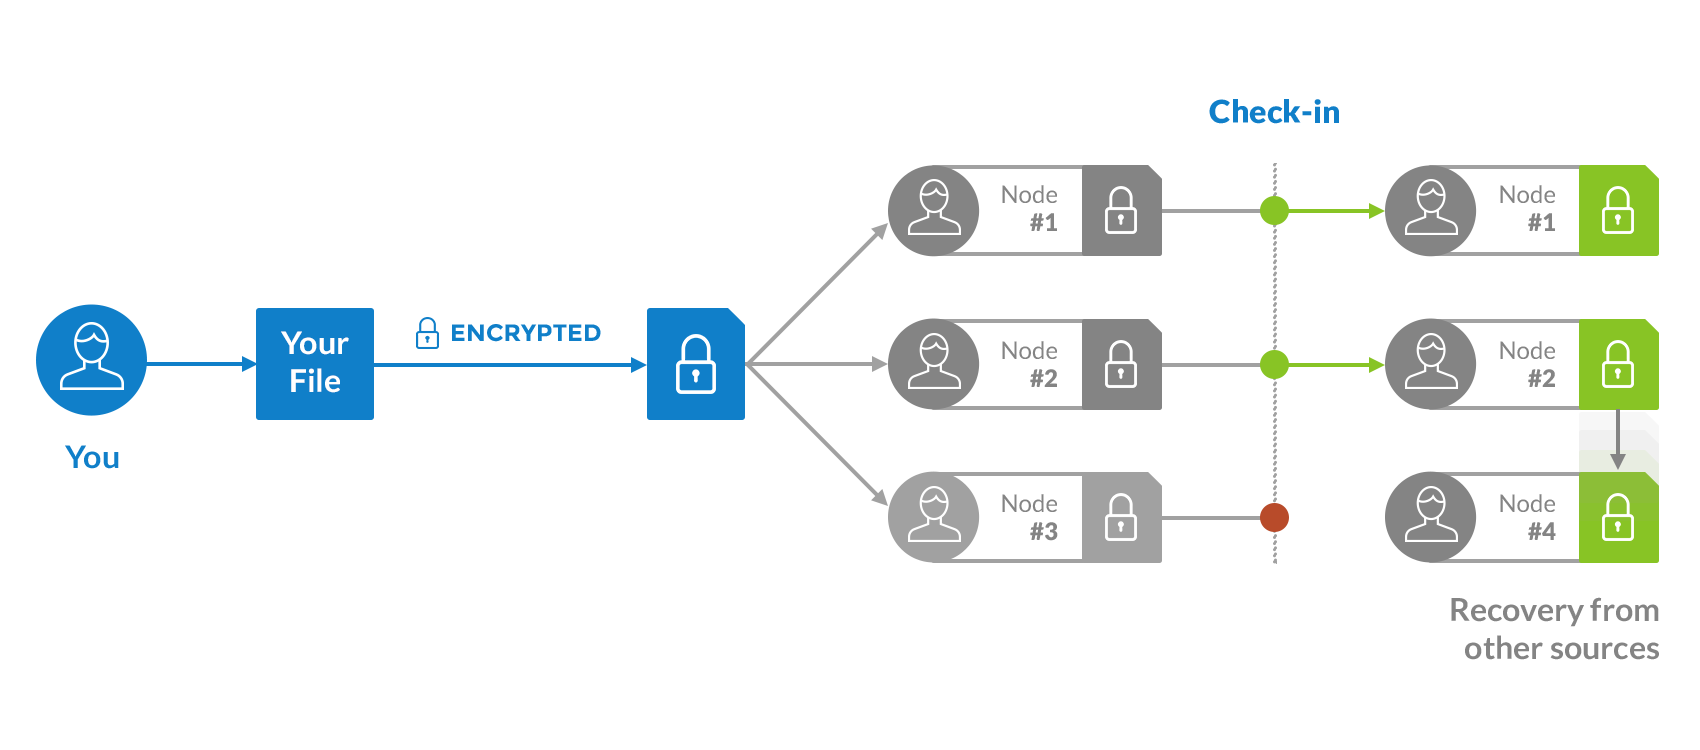
\includegraphics[width=\linewidth]{03}
  \caption{Visualizing the Redundancy Checks }
\end{figure}

\subsection{Bootstrapping}

To quickly get Metadisk up and running, we want to enable the use of existing free and public filehosts as storage providers. Using Plowshare \cite{6}, a command-line (CLI) download/upload tool for popular file sharing websites, we can simplify the task of uploading to these data sources. Pending compatibility with the respective TOS of each, these data sources are free to the Metadisk node with only marginal costs for bandwidth and upkeep for the operation of the node as it shuttles data back and forth between the user and the storage providing hosts.  \\

Free public file-hosts are likely to be quickly outcompeted by local hard disk space. Therefore, we are implementing our own platform called Storj \cite{7} and planning to integrate with another platform called Maidsafe \cite{1}. Both these platforms allow users to offer their own storage space from personal or enterprise computing devices and be part of a decentralized network of storage space. These platforms more directly address problems such as Sybil attacks, redundancy, file integrity, and availability.    \\

It must be clear that Metadisk is platform agnostic. It sees each platform simply as a data source. In this way we can also give end users and applications access to decentralized data platforms through simplified APIs of a Metadisk node. 

\section{Cost Calculations}

As an example test case using the VPS provider Digital Ocean, which could easily host a Metadisk node, we can do some cost estimates. For \$5 per month, we are provided with a maximum of 1 TB of transfer \cite{8}. This works out to approximately \$0.0049 per GB at full utilization. To put this in context, 100 GB would cost us a total of \$1.47 to store, with 3× redundancy, and \$0.49 to fully retrieve.  Dropbox charges \$99/year for that same 100 GB of storage. So in essence, under full utilization of the 100 GB for a year, it would cost \$1.47 plus extra cost for transfer vs. Dropbox’s \$99.  By adopting a pay per usage model, we avoid the user  paying for storage space they don’t actually need.

\begin{figure}[h!]
  \centering
      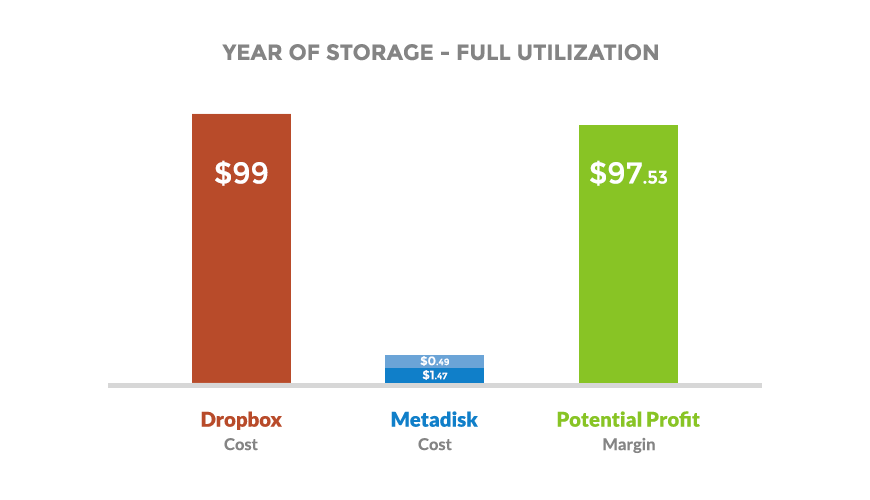
\includegraphics[width=\linewidth]{04}
  \caption{100 GB of Data Storage for 1 Year, Full Utilization. Dark Blue - Storage Costs, Light Blue - Costs for Full Data Retrieval from Metadisk}
\end{figure}


As storage media capacity increases at an exponential rate, doubling every 12 months [17], it has become industry-standard practice for cloud storage providers to store files for long periods of time and continually lower their prices per GB to consumers. Therefore, under our full 100 GB usage example, the cost of \$1.47 per 100 GB for the first year could easily be \$0.74 and approaching zero for the second year and ongoing years. This is competitive with centralized file hosts because even if their cost for storage media halves each year, their ongoing operating costs in data center rents, employee salaries, accounting costs, regulatory burden, legal fees, etc. will remain fixed or increase year over year, limiting their ability to compete with a decentralized model that has no such costs.

\subsection{Reducing Cost and Increasing Profit}

Using unmetered nodes may further reduce the cost for bandwidth, but it is unclear how a hosting provider would respond to the large amounts of data that a Metadisk node could generate. If a node is deleted or destroyed, it has no effect on the network or file availability, so nodes are inherently disposable. This disposability is a cost reducer because there is no need to incur overhead costs insuring against specific node destruction, only continual creation.  \\

An example use case is an unmetered dedicated server provider like Hivelocity \cite{9}.  Their fee for a 1 Gbps unmetered connection allows an estimated 330,000 GB transfer for a total of \$638 per month. Again using 3× redundancy and Dropbox prices, we achieve a gross profit of \$9,166 per month for the node operator. Obviously network congestion and provider hidden caps may limit transfer, but the margins so large that even if the network speed was cut in half we would still be making a substantial profit. \\

To be more fair to the hosting provider and avoid abusing shared hosting providers, another example use case is an unmetered dedicated server provider like Hivelocity \cite{10}.  Their fee for a 1 Gbps unmetered connection allows an estimated 330,000 GB transfer for a total of \$638 per month. Again using 3x redundancy and Dropbox prices, we achieve a gross profit of \$36,666 per month for the node operator. 

\subsection{Ordinary Users and Sunk Costs}

We can also consider the profits of an average residential high speed bandwidth user running their own public Metadisk web node from their personal computer. In this case, the average data speed is 2.0975 MB/s \cite{10}. Using Dropbox prices and a 3× redundancy, this user would see a gross profit of ~\$150 per month. In this case the user has already chosen to pay for the internet connection and personal computer -- these are therefore sunk costs. Marginal costs are quite minimal to such a user considering that extra storage space, electricity, and bandwidth usage are just a small portion of the total cost of their entire home computing budget. This profit potential shall drive Metadisk to create a powerful network effect that benefits all users of the network by bringing cloud storage costs down significantly.\\
 
Many potential residential users might be uncomfortable with the technical aspects of Metadisk. There will be advanced users that will be able to understand the principles of cryptocurrency, but others may not wish to climb that learning curve yet. To allow for rapid network growth and adoption while we wait for mass adoption, we propose designing Metadisk and the distributed storage network so that it can be a lower level service upon which user-friendly higher level abstractions can operate without confusing ordinary users with arcane details.\\
\subsection{Example Service}
An example high level service, which we can choose to call Filebox, would offer similar functionality to a service like Dropbox. Filebox could have its own simplistic cloud storage software, and charge a competitive rate for file storage. On the backend, Filebox could run entirely through Metadisk nodes, eliminating most startup and fixed costs that such a service would otherwise incur. It could purchase credits for its network usage while keeping its own caches of some of the most used files. Filebox would offer much needed abstraction and simplicity to the end user who may not even realize that they are using the Storj network of Metadisk nodes. In return, Filebox would enjoy low market entry costs with an ongoing profit margin over other centralized cloud storage provides. It would only need to maintain the top level software and not the underlying storage hardware.


\begin{figure}[h!]
  \centering
      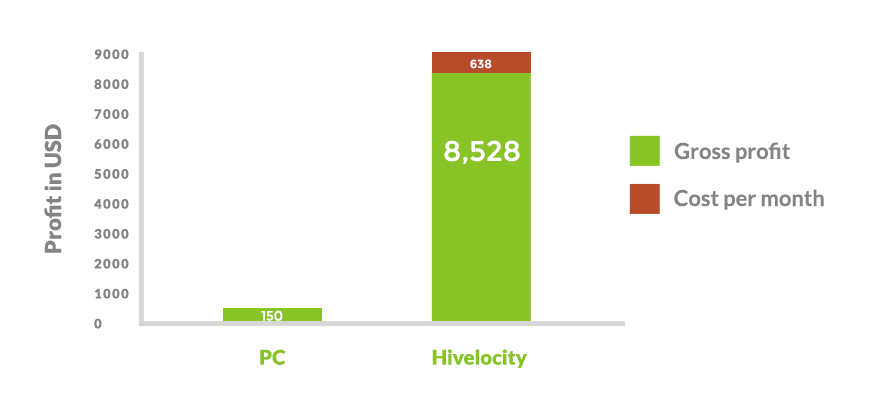
\includegraphics[width=\linewidth]{05}
  \caption{Example Metadisk Node Profits Using Existing Pricing Models and Costless Providers}
\end{figure}


\section{Blockchain as a Metadata Store}

Datacoin \cite{11} is a cryptocurrency whose blockchain is a metadata store for the Metadisk network. This is a temporary measure, and will be replaced at some point with a solution on the Storj platform.  With Datacoin, data is stored in the blockchain forever and can be retrieved using a transaction hash as an identifier \cite{11}. Unfortunately, this leads to a problem known as blockchain bloat. Every full node must store a copy of every transaction in the blockchain. That means with users only storing a few megabytes of data each, the blockchain will quickly scale to an unmanageable size. Just storing a single movie file would cost the uploading user thousands of dollars worth of Datacoin and flood the network. To its credit, once a file is stored on the Datacoin network, it is nearly uncensorable—which may be important for data that must survive—such as an encyclopedia of mathematical principles and scientific knowledge, but is not necessary or scalable for data of a more personal nature.

\subsection{Blockchain Bloat}

Storing the files themselves on the blockchain simply is not possible because of blockchain bloat. We remedy this issue by instead only storing a small amount of metadata information about each file on the blockchain. This is done by sending a simple transaction, with the metadata included. We can store its hash, file location, and any other information that we deem essential. For privacy and security reasons we can encrypt this metadata before we insert it into the blockchain. A sample of this metadata might look something like this:\\

\begin{lstlisting}
{
  version: "0.1",
  datetime: "1391212800",
  filesize: "23124",
  file_hash: "6e163442e29ec8d7538bc86fe2c4a48778e8ae2254632f0889da753b1c357b1b",
   "uploads": [
  { "host_name":"mediafire" , "url":"http://www.mediafire.com/?qorncpzfe74s9"},
  { "host_name":"rapidshare" , "url":"http://rapidshare.com/files/130403982"}
  ]
}
\end{lstlisting}

This sample metadata, regardless of uploaded file size, takes up about 330 bytes of information. We add this to the average transaction, around 500 bytes \cite{12}. Adding some extra padding we get about 1 KB per transaction. In that case, we could store ~1 million files before the metadata in our blockchain reached 1 GB in size. By further refinements we can further minimize the amount of necessary metadata information, using multiple chains, blockchain pruning, and compression,and thereby greatly increase those numbers.

\begin{figure}[h!]
  \centering
      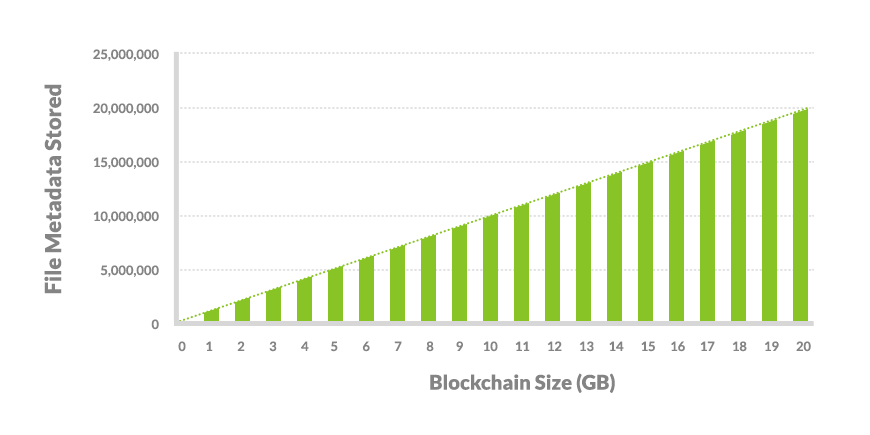
\includegraphics[width=\linewidth]{06}
  \caption{File Metadata Stored vs. Blockchain Sizes}
\end{figure}

\subsection{Further Scaling}

This is indeed reasonable for an initial network of files, but not scalable for a network to handle the full capacity of data of the entire “cloud.” We are bottlenecked by a Satoshi style blockchain’s limitation of 7 transactions per second \cite{13}. As system usage increases we can instead transition to a system where the blockchain stores merkle roots, which are the cryptographic summary of all files being stored in a transaction. In this way, we can prove the existence of millions of files with one transaction. In this way we can directly use the security of the Bitcoin and/or Storj blockchains. At time of writing we are exploring Notary Chains \cite{14} and some other solutions. 

\section{Rewards}

In order to be as decentralized as possible, we separate the reward and payment cryptocurrency from the cryptocurrency that we are using as a data store.The design goal for Storjcoin X, or SJCX, is for it to function as a kind of sound money. To do this, it takes all the code and functionality that has already been developed for Bitcoin (which makes Bitcoin such an excellent form of money) and extends them to provide backing by something of fungible value, cloud storage, to lend that money a soundness beyond mere social acceptance. SJCX will be a deflationary currency by design—over time the amount of cloud storage increments that can be purchased for each SJCX increment will grow as more resources are added to the Storj network, and its value will increase.\\

SJCX will allow users to pay for bandwidth and storage on the Storj distributed storage network through Metadisk portals. The Storj software will act as an autonomous agent market maker setting the price, in SJCX increments, for each storage and bandwidth increment. The Storj software will then pay the providers of storage and bandwidth Storjcoin increments periodically for continuing to provide these resources. Through these programmed automatic behaviours, Storjcoin acts as an autonomous agent providing value and incentives for users and hosting providers to maintain the network. The nature and scope of SJCX is discussed in the Storj whitepaper.

\section{Proof of Resource}
Bandwidth is predicted to become a scarcer resource than storage when we consider Nielsen’s Law \cite{15}, which predicts a doubling every twenty one (21) months of high speed residential internet speeds, as well as Kryder’s Law \cite{16}, which hypothesizes that global storage capacity will continue to double every twelve (12) months.  In order to maintain our development goal of seeing Storjcoin X act as a new form of sound money, we must write the proof of resource functions. As more resource providers connect to the network, the amount of bandwidth-connected storage that a Storjcoin X increment can buy will increase.  In concert with this adjustment of difficulty, the amount of bandwidth-connected storage that a storage provider must connect over a period of time to obtain a Storjcoin X increment will also increase.  \\

This will enable a free market to set the price of SJCX based on the difficulty of obtaining SJCX by providing bandwidth-connected storage hardware to the network, in the same way that Bitcoin prices are in part determined by the cost of mining Bitcoin.  \\

For proof-of-storage, we intend to use the technique of hashing a file plus a seed value to produce a unique hash. One node can prove to another that it holds a particular file by providing the seed, and if that other node has the file it can produce a matching unique hash. The full technical specifications of a proof of resource algorithm is outside the scope of this paper describing Metadisk, and will be further described in the Storj whitepaper.

\section{Conclusion}

We have devised a new model in which a blockchain can serve as the backbone for a distributed application, Metadisk. This application operates autonomously as a peer-to-peer network of nodes running open-source code. We provide a solid introduction to a new type of data platform, but we leave open questions related to dispute mediation, Sybil attacks, and security models underlying the Storj platform.\\

\bibliographystyle{unsrt}
\begingroup
  \raggedright
  \bibliography{meta}
\endgroup


\end{document}